\documentclass{beamer}
\usetheme{Warsaw}
\usepackage{caption}
\usepackage{tikz}
\usepackage{adjustbox}
\usetikzlibrary{arrows.meta, calc, quotes, tikzmark}
\usetikzlibrary{shapes.geometric, arrows, chains, positioning, matrix, fit}

\newcommand{\spike}[2]% #1 = size of spike, #2 = centered text
{\bgroup
	\sbox0{#2}%
	\rlap{\usebox0}%
	\hspace{0.5\wd0}%
	\makebox[0pt][c]{\rule[\dimexpr \ht0+1pt]{0.5pt}{#1}}% top spike
	\makebox[0pt][c]{\rule[\dimexpr -\dp0-#1-1pt]{0.5pt}{#1}}% bottom spike
	\hspace{0.5\wd0}%
	\egroup}


\setbeamerfont{caption}{series=\normalfont,size=\fontsize{7}{9}} 
\newcommand{\matr}[1]{\mathbf{#1}}



\usepackage{stackengine}
\stackMath
\newlength\matfield
\newlength\tmplength
\def\matscale{1.}
\newcommand\dimbox[3]{%
	\setlength\matfield{\matscale\baselineskip}%
	\setbox0=\hbox{\vphantom{X}\smash{#3}}%
	\setlength{\tmplength}{#1\matfield-\ht0-\dp0}%
	\fboxrule=1pt\fboxsep=-\fboxrule\relax%
	\fbox{\makebox[#2\matfield]{\addstackgap[.5\tmplength]{\box0}}}%
}
\newcommand\raiserows[2]{%
	\setlength\matfield{\matscale\baselineskip}%
	\raisebox{#1\matfield}{#2}%
}
\newcommand\matbox[5]{
	\stackunder{\dimbox{#1}{#2}{$\mathbf{#5}$}}{\scriptstyle(#3\times #4)}%
}
\parskip 1em


\title[Flatiron Lesson 2]{Topic Modeling using Non-negative Matrix Factorization (NMF)} 
\subtitle{Tweet topic analysis}

\author{Praveen Gowtham} % Your name


\date{} % Date, can be changed to a custom date


\begin{document}

% Define block styles
\tikzstyle{decision} = [diamond, draw, fill=blue!20, 
text width=4.5em, text badly centered, node distance=3cm, inner sep=0pt]
\tikzstyle{block} = [rectangle, draw, fill=blue!20, 
text width=5em, text centered, rounded corners, minimum height=4em]
\tikzstyle{line} = [draw, -latex']
\tikzstyle{cloud} = [draw, ellipse,fill=red!20, node distance=3cm,
minimum height=2em]
	
	\begin{frame}
		\titlepage % Print the title page as the first slide
	\end{frame}

\begin{frame}{Previously in the land of NLP}
\begin{block}{Text Processing Flow}
	
	\begin{adjustbox}{max totalsize={.9\textwidth}{.7\textheight},center}
		
		\begin{tikzpicture}[auto]
			

			\node [block] (start) {Set of documents};
			
			\node[block, right =1cm of start] (token) {Tokenize};		
			
			\node[block, right =1cm of token] (stopwords) {Remove stop words};
			
			\node[block, right =1cm of stopwords] (lemstem) {Lemmatize or stem};
			
			\node[block, right =1cm of lemstem] (filter) {TF-IDF or Count Vectorizer};
			
			\node[block, right =1cm of filter] (BoW) {Term-frequency matrix (Bag of words)};
			
			
			
			%% paths
			\path[draw,->]
			(start) edge (token)
			(token) edge (stopwords)
			(stopwords) edge (lemstem)
			(lemstem) edge (filter)
			(filter) edge (BoW)
			;
			
		\end{tikzpicture}
		
	\end{adjustbox}

\end{block}
\begin{figure}
	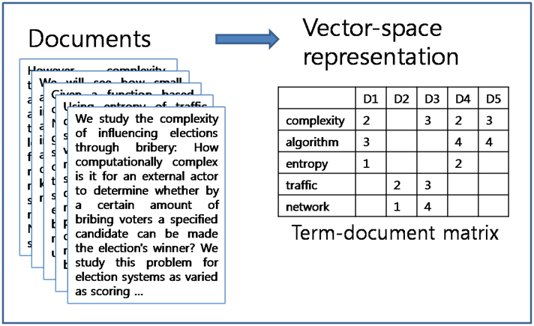
\includegraphics[scale=0.75]{termdoc}
\end{figure}
Previously: Naive Bayes to classify emails as spam or not. 
\end{frame}

\begin{frame}{Other tasks?}
	
\begin{columns}
	\begin{column}{0.5\textwidth}
		\begin{adjustbox}{max totalsize={.5\textwidth}{.7\textheight}, center}
		
		\begin{tikzpicture}[auto]
			
			
			\node [block] (start) {Set of book reviews};
			
	
			\node[ block, right =1cm of start] (topic2) {\textbf{Topic 2} \\body, chop, capo, knife, caught, fishes, sleep casino, FBI, ...};

			\node[block, above = 1cm of topic2] (topic1) {\textbf{Topic 1} \\ knife, onion, parsley, chop, butter, pan, fish, ... };	
			\node[block, below =1cm of topic2] (topic3) {\textbf{Topic 3} \\ ecosystem, anchovy, catch, farming, tuna, fish, sustainable, ...};
			

			%% paths
			\path[draw,->]
			(topic1) edge (start)
			(topic2) edge (start)
			(topic3) edge (start)

			;
			
		\end{tikzpicture}
		
	\end{adjustbox}
\end{column}
\begin{column}{0.5\textwidth}
	\begin{itemize}
		\item Collection of book reviews: combinations of 3 topics.
		\item Certain word sets feature heavily in each topic.
		\item Take a book review: get combination of topics.
	\end{itemize}
\end{column}
\end{columns}

\end{frame}

\begin{frame}{Other tasks?}
	
	\begin{columns}
		\begin{column}{0.5\textwidth}
			\begin{adjustbox}{max totalsize={.5\textwidth}{.7\textheight}, center}
				
				\begin{tikzpicture}[auto]
					
					
					\node [block] (start) {Set of book reviews};
					
					
					\node[ block, right =1cm of start] (topic2) {\textbf{Topic 2} \\body, chop, capo, knife, caught, fishes, sleep casino, FBI, ...};
					
					\node[block, above = 1cm of topic2] (topic1) {\textbf{Topic 1} \\ knife, onion, parsley, chop, butter, pan, fish, ... };	
					\node[block, below =1cm of topic2] (topic3) {\textbf{Topic 3} \\ ecosystem, anchovy, catch, farming, tuna, fish, sustainable, ...};
					
					
					%% paths
					\path[draw,->]
					(topic1) edge (start)
					(topic2) edge (start)
					(topic3) edge (start)
					
					;
					
				\end{tikzpicture}
				
			\end{adjustbox}
		\end{column}
		\begin{column}{0.5\textwidth}
			\begin{figure}
			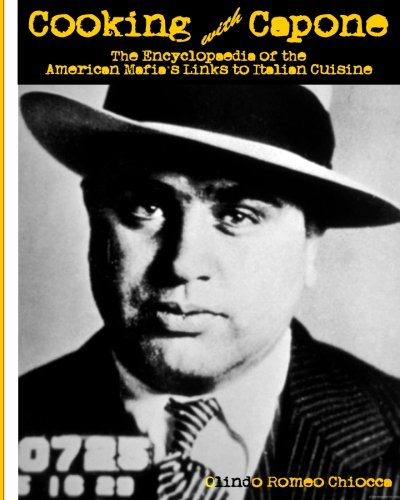
\includegraphics[scale=0.21]{capone}
			\end{figure}
		
			\begin{figure}
			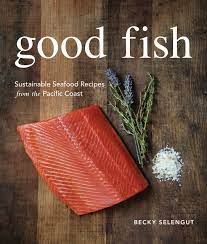
\includegraphics[scale=1]{fish_sustainable}
			\end{figure}

		\end{column}
	\end{columns}
	
\end{frame}

\begin{frame}{Other tasks?}
	
	\begin{columns}
		\begin{column}{0.5\textwidth}
			\begin{adjustbox}{max totalsize={.5\textwidth}{.7\textheight}, center}
				
				\begin{tikzpicture}[auto]
					
					
					\node [block] (start) {Set of book reviews};
					
					
					\node[ block, right =1cm of start] (topic2) {\textbf{Topic 2} \\body, chop, capo, knife, caught, fishes, sleep casino, FBI, ...};
					
					\node[block, above = 1cm of topic2] (topic1) {\textbf{Topic 1} \\ knife, onion, parsley, chop, butter, pan, fish, ... };	
					\node[block, below =1cm of topic2] (topic3) {\textbf{Topic 3} \\ ecosystem, anchovy, catch, farming, tuna, fish, sustainable, ...};
					
					
					%% paths
					\path[draw,->]
					(topic1) edge (start)
					(topic2) edge (start)
					(topic3) edge (start)
					
					;
					
				\end{tikzpicture}
				
			\end{adjustbox}
		\end{column}
		\begin{column}{0.5\textwidth}
		\begin{figure}
			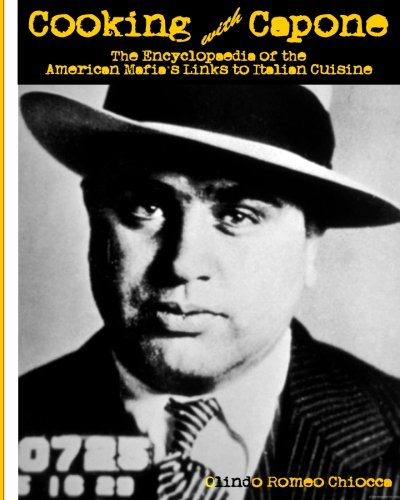
\includegraphics[scale=0.21]{capone}
		\end{figure}
	$$0.5 Topic1 + 0.5Topic2 $$
		\end{column}
	\end{columns}
	
\end{frame}

\begin{frame}{Other tasks?}
	
	\begin{columns}
		\begin{column}{0.5\textwidth}
			\begin{adjustbox}{max totalsize={.5\textwidth}{.7\textheight}, center}
				
				\begin{tikzpicture}[auto]
					
					
					\node [block] (start) {Set of book reviews};
					
					
					\node[ block, right =1cm of start] (topic2) {\textbf{Topic 2} \\body, chop, capo, knife, caught, fishes, sleep casino, FBI, ...};
					
					\node[block, above = 1cm of topic2] (topic1) {\textbf{Topic 1} \\ knife, onion, parsley, chop, butter, pan, fish, ... };	
					\node[block, below =1cm of topic2] (topic3) {\textbf{Topic 3} \\ ecosystem, anchovy, catch, farming, tuna, fish, sustainable, ...};
					
					
					%% paths
					\path[draw,->]
					(topic1) edge (start)
					(topic2) edge (start)
					(topic3) edge (start)
					
					;
					
				\end{tikzpicture}
				
			\end{adjustbox}
		\end{column}
		\begin{column}{0.5\textwidth}
			\begin{figure}
				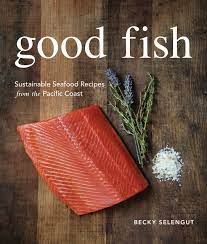
\includegraphics[scale=1]{fish_sustainable}
			\end{figure}
			$$ 0.7 Topic1 + 0.3 Topic3 $$
		\end{column}
	\end{columns}
\end{frame}

\begin{frame}{Topic Modeling: the problem}
		\begin{columns}
		\begin{column}{0.5\textwidth}
			\begin{adjustbox}{max totalsize={.5\textwidth}{.7\textheight}, center}
				
				\begin{tikzpicture}[auto]
					
					
					\node [block] (start) {Term-document matrix};
					
					
					\node[ block, right =1cm of start] (topic2) {$ \vdots$};
					
					\node[block, above = 1cm of topic2] (topic1) {\textbf{Topic 1} \\ ? };	
					\node[block, below =1cm of topic2] (topic3) {\textbf{Topic K} \\ ?};
					
					
					%% paths
					\path[draw,->]
					(topic1) edge (start)
					(topic2) edge (start)
					(topic3) edge (start)
					
					;
					
				\end{tikzpicture}
				
			\end{adjustbox}
		\begin{itemize}
		\item K "latent" topics. 
		\item Unknown word distribution for topics.
		\end{itemize}
		\end{column}
		\begin{column}{0.5\textwidth}
			\begin{adjustbox}{max totalsize={.5\textwidth}{.7\textheight}, center}
	
	\begin{tikzpicture}[auto]
		
		
		\node [block] (start) {Document};
		
		
	\end{tikzpicture}
	
\end{adjustbox}
			$$ ? Topic1 + \hdots + ? TopicK $$
					\begin{itemize}
				\item Document topic breakdown: unknown.
			\end{itemize}
		\end{column}
	\end{columns}

\end{frame}
\begin{frame}{Topic Modeling: the problem}
	\begin{columns}
		\begin{column}{0.5\textwidth}
			\begin{adjustbox}{max totalsize={.5\textwidth}{.7\textheight}, center}
				
				\begin{tikzpicture}[auto]
					
					
					\node [block] (start) {Term-document matrix};
					
					
					\node[ block, right =1cm of start] (topic2) {$ \vdots$};
					
					\node[block, above = 1cm of topic2] (topic1) {\textbf{Topic 1} \\ ? };	
					\node[block, below =1cm of topic2] (topic3) {\textbf{Topic K} \\ ?};
					
					
					%% paths
					\path[draw,->]
					(topic1) edge (start)
					(topic2) edge (start)
					(topic3) edge (start)
					
					;
					
				\end{tikzpicture}
				
			\end{adjustbox}
			\begin{itemize}
				\item K "latent" topics. 
				\item Unknown word distribution for topics.
			\end{itemize}
		\end{column}
		\begin{column}{0.5\textwidth}
			\begin{adjustbox}{max totalsize={.5\textwidth}{.7\textheight}, center}
	
	\begin{tikzpicture}[auto]
		
		
		\node [block] (start) {Document};
		
		
	\end{tikzpicture}
	
\end{adjustbox}
			$$ ? Topic1 + \hdots + ? TopicK $$
			\begin{itemize}
				\item Document topic breakdown: unknown.
			\end{itemize}
		\end{column}
	\end{columns}
	\begin{center}
		\textcolor{red}{Goal is to learn both sides of this at the same time.}
	\end{center}
\end{frame}
\begin{frame}{Non-negative Matrix Factorization: NMF}

$$\renewcommand\matscale{.6}
\matbox{7}{4}{N_{term}}{N_{doc}}{X} \approx 
\matbox{7}{2}{N_{term}}{K}{W} \raiserows{2.5}{\matbox{2}{4}{K}{N_{doc}}{H}} $$

\begin{block}{Definitions}	
$\matr{X}$: word frequency for the documents (our BoW matrix)\\
$\matr{W}$: word distribution for each topic. \\
$\matr{H}$: weight of each topic in a document \\	
\end{block}
\end{frame}

\begin{frame}{Non-negative Matrix Factorization: NMF}
	
	$$\renewcommand\matscale{.6}
	\matbox{7}{4}{N_{term}}{N_{doc}}{X} \approx 
	\matbox{7}{2}{N_{term}}{K}{W} \raiserows{2.5}{\matbox{2}{4}{K}{N_{doc}}{H}} $$
	
	\begin{block}{Conditions}
		\begin{itemize}	
		\item Assumes data generated by K topics.
		\item \textbf{W} and \textbf{H} are non-negative matrices.
		\end{itemize}
	\end{block}

\end{frame}
\begin{frame}{NMF: Some Intuition}
	Each column of \textbf{X}: term frequencies for a given document.
	\begin{figure}
			\begin{center}
			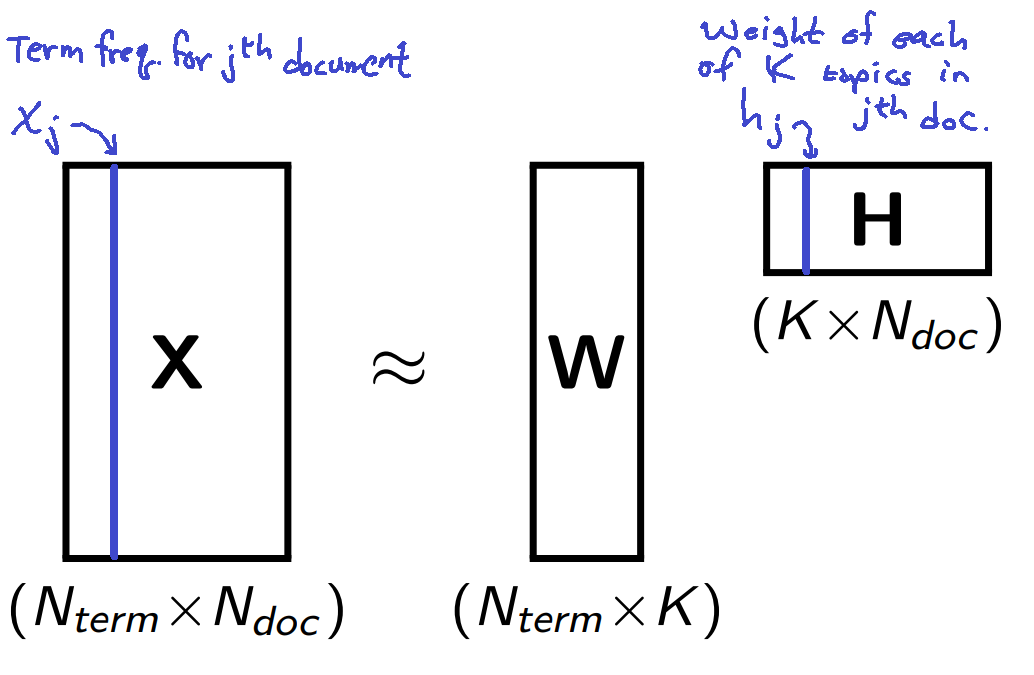
\includegraphics[scale = 0.6]{doctermdecomp}
		\end{center}
	\end{figure}


\end{frame}
\begin{frame}{NMF: Some Intuition}
	Each column of \textbf{X}: term frequencies for a given document.
	\begin{figure}
		\begin{center}
			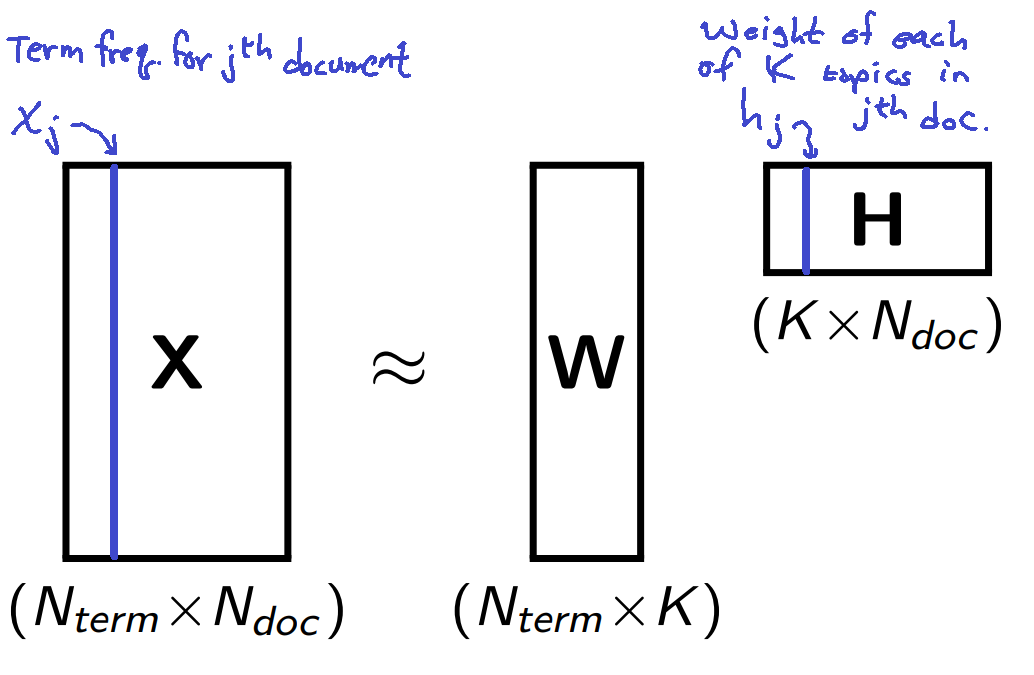
\includegraphics[scale = 0.4]{doctermdecomp}
		\end{center}
	\end{figure}
Short form:
	$$x_j \approx \textbf{W}\begin{bmatrix}
	h^{doc(j)}_{topic(1)} \\
	\vdots \\
	h^{doc(j)}_{topic(K)}
\end{bmatrix}
$$

\end{frame}
\begin{frame}{NMF: Some Intuition}
	\[
x_j \approx \begin{bmatrix}
	\spike{30pt}{$w^{topic(1)}$}  & \spike{30pt}{$w^{topic(2)}$} & \hdots & \spike{30pt}{$w^{topic(K)}$}
\end{bmatrix}
\begin{bmatrix}
	h^{doc(j)}_{topic(1)} \\
	\vdots \\
	h^{doc(j)}_{topic(K)}
\end{bmatrix}
\]
\end{frame}
\begin{frame}{NMF: Some Intuition}
	Expanding it:

$$x_j \approx h_{topic(1)}^{document(j)}*\begin{bmatrix}
	w_{1}^{topic(1)} \\
	w_{2}^{topic(1)} \\
	\vdots \\
	w_{N_{term}}^{topic(1)}
\end{bmatrix} + \hdots + h_{topic(K)}^{document(j)}*\begin{bmatrix}
w_{1}^{topic(K)} \\
w_{2}^{topic(K)} \\
\vdots \\
w_{N_{term}}^{topic(K)}
\end{bmatrix} $$
\begin{block}{In words:}
Tries to model term frequencies for each document as weighted sum of word distributions for each topic.
\end{block}
\end{frame}

\begin{frame}{Finding W and H}
	One possible way: minimize squared loss error for each element.
	$$ L = \sum_{ij}|X_{ij} - (\textbf{W}\textbf{H})_{ij}|^2 $$
	subject to all elements of W and H $\geq 0$.
	\begin{block}{Result}
		Minimizing loss subject to constraint:
		\begin{itemize}
			\item Often leads to topics that are interpretable. (\textbf{W} matrix) 
			\item Topic breakdown for each document. (\textbf{H} matrix) 
		\end{itemize}
	\end{block}

D.D. Lee and H.S. Seung, Nature \textbf{401}, 789 (1999)
\end{frame}
\begin{frame}{Case Study: COVID-19 Tweet Analysis}
\begin{columns}
\begin{column}{0.5\textwidth}
Think tank hires you:
\begin{itemize}
	\item Want to know trending concerns about Covid-19.
	\item Higher level analytics on these concerns.
	\begin{itemize}
		\item Distribution of concerns/issues.
		\item Concerns/issues that go hand-in-hand
		\item Issue importance time trends.
	\end{itemize} 
\item Take to the Twitter-verse.
\end{itemize}
\end{column}
\begin{column}{0.5\textwidth}
\begin{figure}
	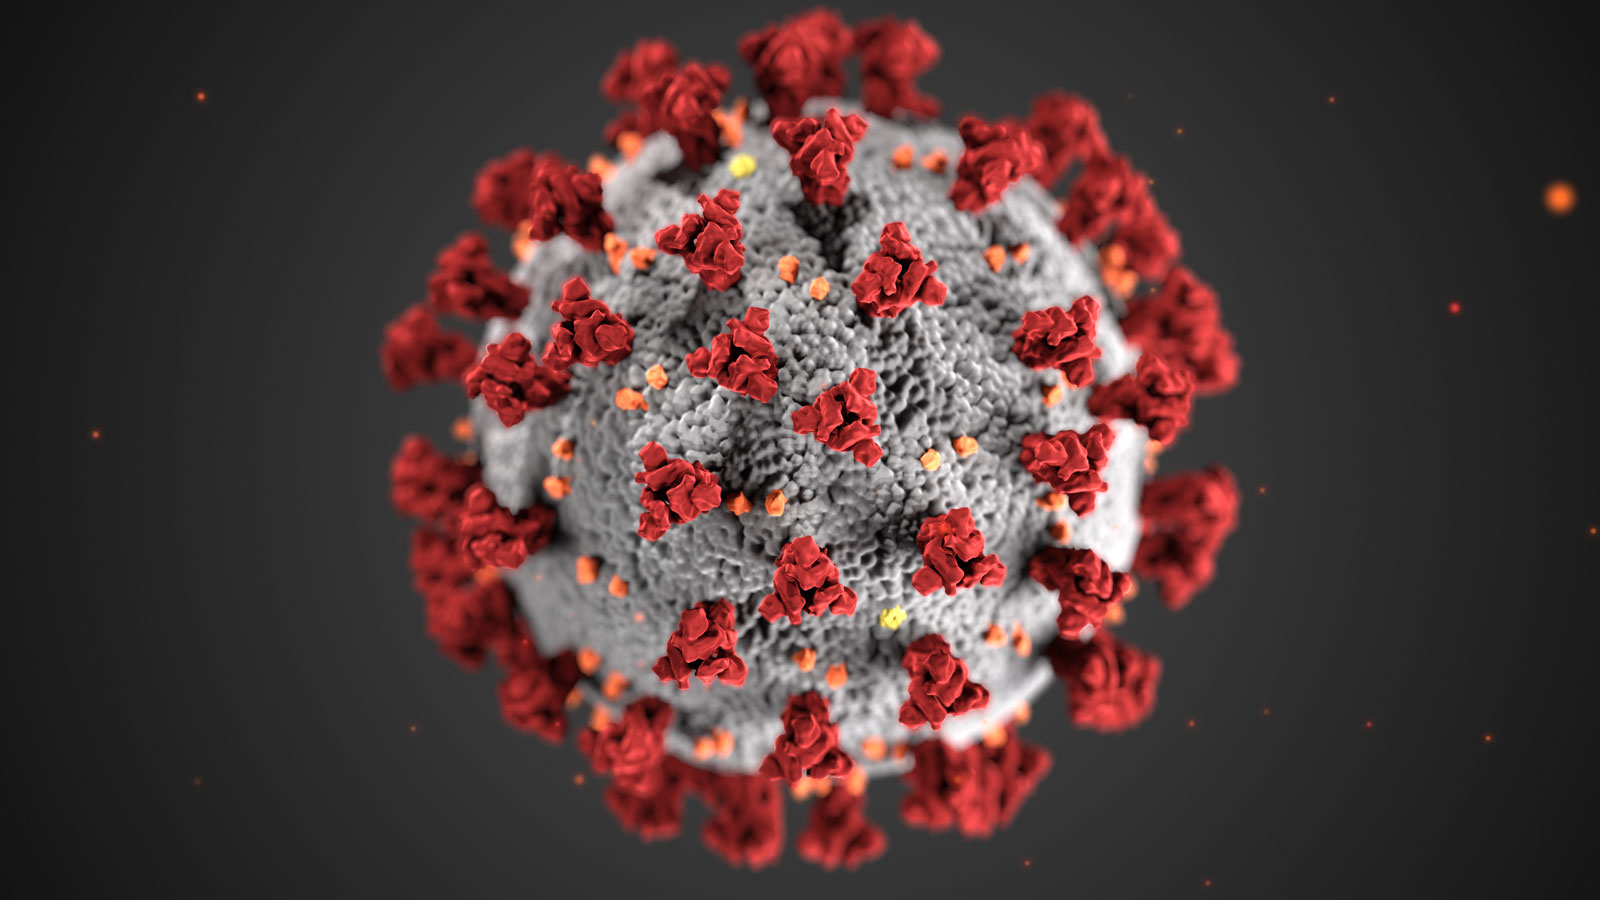
\includegraphics[scale=0.09]{covid19}
	\caption{COVID-19}
\end{figure}
\begin{block}{Starting point}
	Topic modeling of Covid-19 tweets using NMF.
\end{block}
\end{column}
\end{columns}
\end{frame}
\end{document}